\newpage
\subsection{Caso d'uso UC11: Visualizzazione pagina utente}
\label{UC11}
\begin{figure}[h]
	\centering
	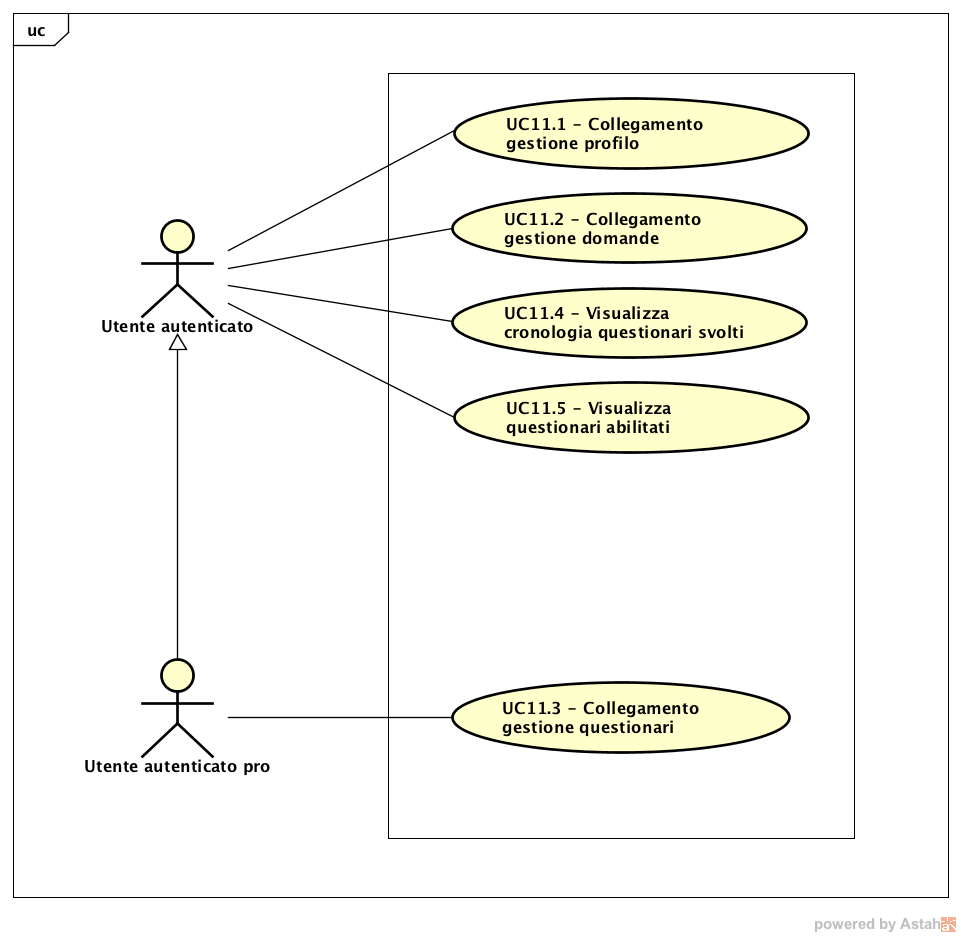
\includegraphics[scale=0.5]{UML/UC11.png}
	\caption{UC11: Gestione pagina utente}
\end{figure}

\begin{itemize}
\item\textbf{Attori}: utente autenticato, utente autenticato pro;
\item\textbf{Descrizione}: gli attori da questa pagina possono: 
\begin{itemize}
	\item Visualizzare tutti i dati del loro profilo;
	\item Visualizzare le statistiche dei questionari svolti;
	\item Visualizzare la cronologia dei questionari svolti;
	\item Accedere alla parte del sistema che permette di modificare il profilo;
	\item Accedere alla parte del sistema che permette l'aggiunta di nuove domande;
	\item Accedere alla parte del sistema che permette la creazione di questionari.
\end{itemize}
\item\textbf{Precondizione}: gli attori sono entrati nella pagina di visualizzazione del profilo e il sistema è pronto per mostrare i dati;
\item\textbf{Postcondizione}: gli attori hanno visualizzato i loro dati come richiesto al sistema;
\item\textbf{Scenario principale}:
\begin{itemize}
\item Gli attori hanno scelto di andare alla pagina di gestione del profilo (UC11.1);
\item Gli attori hanno scelto di andare alla pagina di gestione delle domande (UC11.2);  
\item Gli attori hanno scelto di andare alla pagina di gestione dei questionari (UC11.3);
\item Gli attori hanno scelto di andare alla pagina di visualizzazione della cronologia dei questionari svolti (UC11.4);
\item Gli attori hanno scelto di visualizzare le statistiche di un questionario (UC11.4.1);
\item Gli attori hanno scelto di andare alla pagina di visualizzazione dei questionari abilitati (UC11.5);
\item Gli attori hanno selezionato un questionario abilitato (UC11.5.1);
\end{itemize}
\item\textbf{Inclusioni}: Viene incluso l'UC7 per la compilazione dei questionari.
\end{itemize}

\subsubsection{Caso d'uso UC11.1: Collegamento gestione profilo}
\begin{itemize}
\item\textbf{Attori}: utente autenticato, utente autenticato pro;
\item\textbf{Descrizione}: gli attori vengono portati nella pagina di gestione del profilo dove potranno modificare liberamente tutti i loro dati;
\item\textbf{Precondizione}: gli attori hanno premuto l'apposito link di gestione del profilo;
\item\textbf{Postcondizione}: il sistema ha portato gli attori alla pagina di gestione del profilo;
\item\textbf{Scenario principale}: gli attori si trovano nella pagina di gestione del profilo e potranno attuare tutte le modifiche desiderate;
\end{itemize}

\subsubsection{Caso d'uso UC11.2: Collegamento gestione delle domande}
\begin{itemize}
\item\textbf{Attori}: utente autenticato, utente autenticato pro;
\item\textbf{Descrizione}: gli attori vengono portati nella pagina di gestione delle domande dove potranno inserire o modificare le loro domande;
\item\textbf{Precondizione}: gli attori hanno premuto l'apposito link di gestione delle domande;
\item\textbf{Postcondizione}: il sistema ha portato gli attori alla pagina di gestione delle domande;
\item\textbf{Scenario principale}: gli attori si trovano nella pagina di gestione delle domande e potranno attuare tutte le modifiche desiderate;
\end{itemize}

\subsubsection{Caso d'uso UC11.3: Collegamento gestione questionari}
\begin{itemize}
\item\textbf{Attori}: utente autenticato, utente autenticato pro;
\item\textbf{Descrizione}: gli attori vengono portati nella pagina di gestione dei questionari dove potranno compiere tutte le azioni possbili sui questionari;
\item\textbf{Precondizione}: gli attori hanno premuto l'apposito link di gestione dei questionari;
\item\textbf{Postcondizione}: il sistema ha portato gli attori alla pagina di gestione dei questionari;
\item\textbf{Scenario principale}: gli attori si trovano nella pagina di gestione dei questionari e potranno attuare tutte le modifiche desiderate;
\end{itemize}

\subsubsection{Caso d'uso UC11.4: Visualizzazione cronologia questionari svolti}
\label{UC11.4}
\begin{figure}[h]
	\centering
	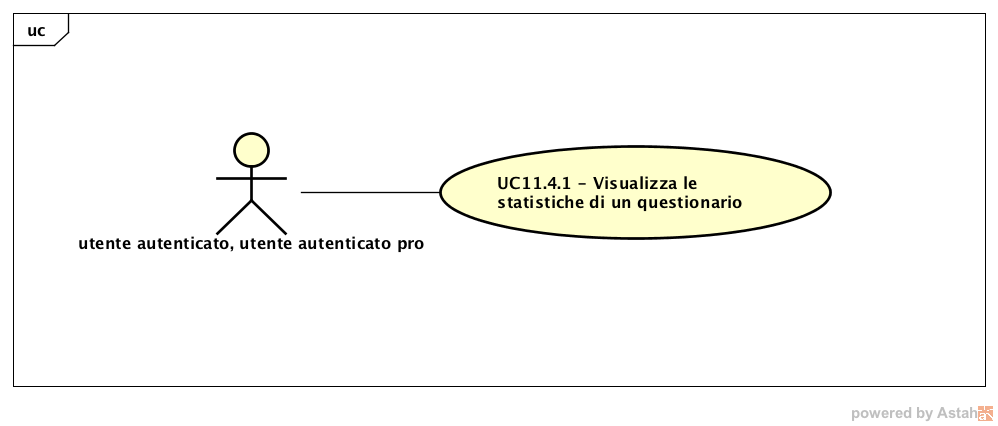
\includegraphics[scale=0.5]{UML/UC11_4.png}
	\caption{UC11.4: Visualizzazione cronologia questionari svolti}
\end{figure}
\begin{itemize}
\item\textbf{Attori}: utente autenticato, utente autenticato pro;
\item\textbf{Descrizione}: gli attori possono visualizzare la cronologia dei questionari svolti;
\item\textbf{Precondizione}: gli attori hanno compilato almeno un questionario;
\item\textbf{Postcondizione}: il sistema ha mostrato agli attori la cronologia dei questionari;
\item\textbf{Scenario principale}: gli attori richiedono la visualizzazione della cronologia dei questionari da loro eseguiti.
\end{itemize}

\subsubsection{Caso d'uso UC11.4.1: Visualizza le statistiche di un questionario scelto}
\begin{itemize}
\item\textbf{Attori}: utente autenticato, utente autenticato pro;
\item\textbf{Descrizione}: gli attori possono visualizzare le statistiche di un questionario da loro scelto fra quelli presenti nella loro cronologia;
\item\textbf{Precondizione}: gli attori devono aver selezionato un questionario tra quelli presenti nella cronologia;
\item\textbf{Postcondizione}: il sistema ha mostrato agli attori le statistiche del questionario selezionato;
\item\textbf{Scenario principale}: gli attori si trovano nella pagina dedicata alla visualizzazione delle statistiche di un particolare questionario da loro scelto.
\end{itemize}

\subsubsection{Caso d'uso UC11.5: Visualizza questionari abilitati}
\label{UC11.5}
\begin{figure}[h]
	\centering
	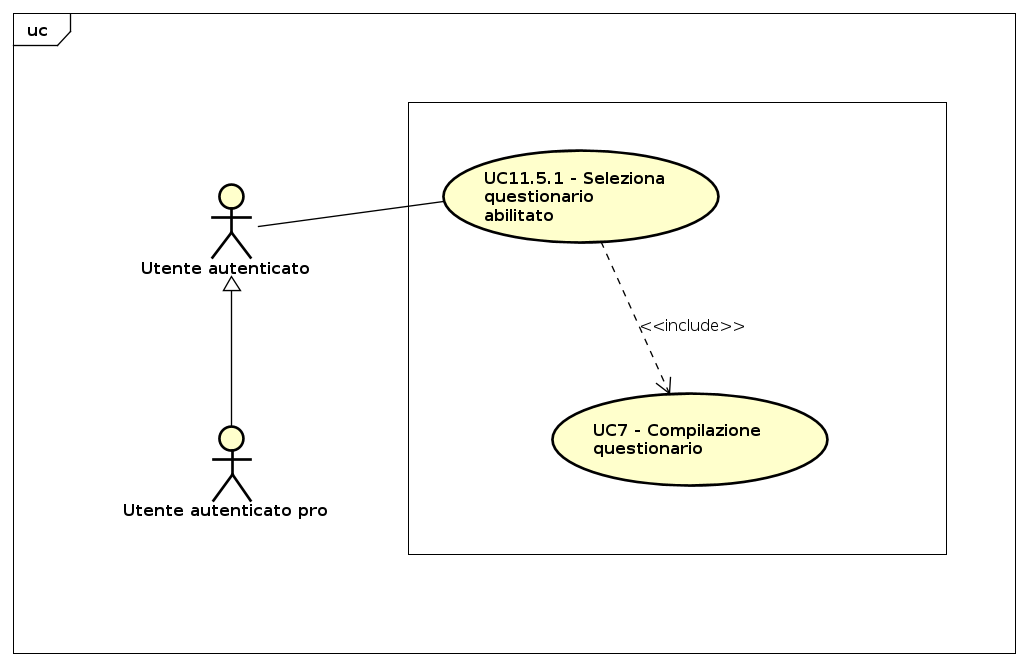
\includegraphics[scale=0.5]{UML/UC11_5.png}
	\caption{UC11.5: Visualizza questionari abilitati}
\end{figure}
\begin{itemize}
\item\textbf{Attori}: utente autenticato, utente autenticato pro;
\item\textbf{Descrizione}: gli attori possono visualizzare la lista dei questionari a cui sono stati abilitati da parte dell'utente autenticato pro proprietario del questionario.
\item\textbf{Precondizione}: gli attori devono aver richiesto l'abilitazione ad un questionario e devono essere stati accettati dal proprietario;
\item\textbf{Postcondizione}: il sistema ha mostrato agli attori tutti i questionari a cui sono stati abilitati;
\item\textbf{Scenario principale}: gli attori richiedono la visualizzazione dei questionari a cui sono stati abilitati da parte del proprietario. 
\end{itemize}

\subsubsection{Caso d'uso UC11.5.1: Seleziona questionario abilitato}
\begin{itemize}
\item\textbf{Attori}: utente autenticato, utente autenticato pro;
\item\textbf{Descrizione}: gli attori possono selezionare un questionario a cui sono stati abilitati ed eseguirlo;
\item\textbf{Precondizione}: gli attori devono essere stati abilitati ad almeno un questionario;
\item\textbf{Postcondizione}: gli attori hanno selezionato un questionario a cui sono stati abilitati e il sistema è pronto per farlo eseguire;
\item\textbf{Scenario principale}: gli utenti richiedono di eseguire un questionario a cui sono stati abilitati.
\end{itemize}